\section[Aplikace ionizujícího záření v geologii a geofyzice]{Aplikace ionizujícího záření v geologii a geofyzice}

\subsection{Radiometrické datování hornin}

\textbf{Uran -- olovo:}

= Výhradně pro vulkanické horniny, k datování se používá Zr $\rightarrow$ ZrSiO$_4$.

\begin{itemize}
    \item[1)] Máme zirkon ZrSiO$_4$, který obsahuje malé množství U-238 a U-235.
    \item[2)] Dochází k jejich rozpadu $\rightarrow$ vznik stabilních izotopů olova.
    \item[3)] Zirkon krystalizuje z magmatu $\rightarrow$ silně vytlačuje veškeré olovo -$\rightarrow$ předpoklad: po vyvření není ve vyvřelině žádné olovo $\rightarrow$ uzavřený systém pro U i Pb.    
    \item[4)] Jakékoliv olovo, co je detekováno, poté odpovídá rozpadu uranu (tzv. radiogenní olovo).
    \item[5)] Určí se poměr U/Pb $\rightarrow$ hmotnostní spektrometrie .
\end{itemize}

\textbf{Burial dating method -- Al a Be:}

\begin{itemize}
    \item[1)] Máme kosmogenní izotopy $^{26}$Al a $^{10}$Be -- vznik interakcí kosmického záření -- akumulace v horninách jako křemen
    \item[2)] Vznikne zhrubaa konstantní poměr $^{26}$Al a $^{10}$Be .
    \item[3)] Po pohřbení $\rightarrow$ odstínění od kosmického záření $\rightarrow$ poločas hliníku: 729 000 let, u beryllia: 1,39 milionů let $\rightarrow$ hliník se rozpadá rychleji .
    \item[4)] Z poměru můžu určit stáří.
    \item[5)] Limitace na látky obsahující křemen, stáří v stovkách tisíc až milionech let.
\end{itemize}

\textbf{Letecké monitorování} = spektrometrické měření záření gama ze svrchní vrstvy půdy. Umožňuje získat informace o vlastnostech hornin a půd a zejména o jejich obsahu přírodních radionuklidů (především K, U, Th).

Můžu využít i při vyhledávání ložisek uranu, měření v dolech. Dále lze gamma spektrometrii využít v závodě na zpracování uranu, kde jsou jednotlivé vozíky/haldy uranu rozřazovány podle intenzity záření.

Ve stavebnictví využívám při měření radonu. Ten kromě jiného může být měřen při vyhledávání zlomů v půdě, neboť cestuje vzhůru právě skrz zlomy.

\subsection{Jaderná karotáž (well logging)}

Karotáž je metoda v geofyzice, která se používá k měření fyzikálních vlastností hornin v podzemí, zejména při průzkumu a těžbě ropy a zemního plynu. Radiometrická karotáž je jedním z typů této metody, která využívá radioaktivních vlastností hornin.

Princip spočívá v detekci a měření radioaktivního záření emitovaného horninami. Toto záření pochází z přirozeně se vyskytujících radioaktivních prvků, jako jsou uran, thorium a K-40, které jsou součástí hornin. Tyto prvky emitují gama záření, které lze detekovat a měřit pomocí vhodných detektorů umístěných na vrtacích zařízeních.

Při radiometrické karotáži se na vrtací nástroje (karoty) umístí detektory, které registrují gama záření vysílané z hornin. Intenzita tohoto záření může poskytnout informace o složení hornin. Například vysoký obsah uranu může indikovat přítomnost uranových rud, což může být důležité pro průzkum ložisek uranu.

\textbf{Nuclear borehole logging} (jaderná karotáž) je metoda, která využívá velké prostupnosti neutronů a gama záření. Využívá se v průmyslu pro ropu, zemní plyn a uran. Jedná se o metody, které umožňují detekci nestabilních izotopů, a nebo metody, které takovéto izotopy vytváří, což se pak detekuje. Výhodou je dobrá penetrace záření, díky čemuž záření snadno projde skrze obalové materiály. Tyto metody je možné využívat i pokud je vrt vyplněn kapalinou. 

Metody:

\begin{itemize}
    \item \textbf{Gama karotáž}: Nejvíce využívané, jedná se o pasivní metodu. V zásadě jen přijímáme měření. Nejčastější aplikace je v lithologii (nauka o výzkumu a popisu usazených hornin) a v stratigrafii (určování stáří hornin). Zaznamenává se celkové gama záření detekované ve vrtu, neboli expoziční příkon v hornině, či stanovení obsahu jednotlivých radioaktivních prvků v rudním průzkumu. 
    
    Hlavní radioizotopy: thorium (Th-230 a Th-232), draslík (K-40) a uran (U-235 a U-238).
    
    Pokud signál je zesílený $\rightarrow$ asi břidlice, pokud zeslabený $\rightarrow$ pískovec, vápenec, dolomit -- můžu mít ještě spektrální gamma karotáž, čímž stanovím obsah radioaktivních prvků ve vrtu.

    \item \textbf{Gama-Gama karotáž}: Jedná se o aktivní metodu, kde je potřeba učinit nějakou "akci". Gama záření je vyzářeno ze zdroje v zavedené sondě ve vrtu. Toto záření pak prochází okolníma šutrama, interaguje, a pomocí Comptonova rozptylu je zpětně detekováno v detektorech, které se taktéž nachází v zavážené sondě. Výsledkem je stanovení hustoty, pórovitosti atd.
    
    Platí totiž, že odezva bude nepřímo úměrná elektronové hustotě. Detektor v karotážní sondě měří intenzitu gama záření, které se vrací k sondě po interakci s horninou. Nižší intenzita detekovaného záření indikuje vyšší hustotu horniny, protože více záření bylo rozptýleno nebo absorbováno. Naopak vyšší intenzita naznačuje nižší hustotu horniny. 
    
    Druhá možná varianta je detekce sekundárního záření vzniklé fotoefektem, čímž se stanovuje obsah těžkých prvků jako Ba, Sb, Pb. Zdrojem gama záření je často Cs-137. Detektory jsou vhodně odstíněny od zářiče.

    \item \textbf{Neutronová karotáź}: Obsahuje neutronový zdroj v zavedené sondě a detektory pro záznam interakcí, ke kterým dochází v blízkosti vrtu, do kterého je sonda zavedená. Emitované vysokoenergetické neutrony jsou postupně zpomalovány (nejvíce na jádrech vodíku) a následně mohou být absorbovány v materiálu a nebo v detektoru neutronů. Proto lze hovořit o \textbf{neutron-gama karotáži} (měřím charakteristické gamma vzniklé při interakci neutronu s horninou) a o \textbf{neutron-neutron karotáži}, kdy detekuji zpomalené tepelné neutrony, které difundovaly až k detektoru. Většina těchto interakcí závisí na množství přítomného vodíku, a tedy i vody v šutrácích, které jsme provrtali při vrtání vrtu. Nejčastější zdroj vysokoenergetických neutronů je AmBe.

    Neutronová karotáž je obecně souhrn pro neutron-neutron karotáž (zdroj rychlých neutronů $\rightarrow$ zpomalení v hornině $\rightarrow$ stanovení pórovitosti hornin (zpomalení na vodíku)). Dále sem patří neutron-gama karotáž (radiační záchyt neutronů, stanovení pórovitosti, rozhraní plyn-ropa a plyn-voda a také některých prvků Cl, Ni, Fe, Cu, Ti, Mn) a na závěr sem patří Neutronová aktivační karotáž (v podstatě aktivační analýza a měříme charakteristické záření vzniklého radioaktivního izotopu $\rightarrow$ stanovení Cu, Mn, Al, Si, F).
    
% V geologickém průzkumu se už dávno využívá tzv. radioaktivní karotáž. při ní se do geologického vrtu nejprve spustí
% sonda s neutronovým zářičem a poté se měří sekundární radioaktivita geologických vrstev, vyvolaná tokem neutronů.
% Měřením aktivity plynných radionuklidů v půdě se určuje stáří geologických vrstev, rozptylem neutronů se měří vlhkost
% půdy nebo přítomnost zdrojů podzemní vody či ropy

\end{itemize}

Vodohospodáři využívají radionuklidy k měření průtoků v řekách i vodovodních potrubích. Do vody nebo vodního toku je vstříknut radioizotop (bez zátěže ŽP) a následně je tento izotop detekován v místě s různými detektory (můžou být různě podél břehu i v hloubce). Na základě času a koncentrace lze stanovit průtok. Používám, když nemohu použít standardní metody. 

Rozlišuji:

\begin{itemize}
    \item metodu časové distribuce -- sleduji za jak dlouho se mi vzorek dopravil z bodu A do bodu B a v jaké koncentraci,
    \item metodu ředění -- podle toho, jak se koncentrace v toku mění, určím průtok.
\end{itemize}

Ozařováním je možno ošetřit také odpadní vody obsahující některé nebezpečné látky ještě před přivedením do běžných čističek odpadních vod. Zářiče s radiokobaltem zabraňují množení nežádoucích mikroorganizmů, které snižují kvalitu pitné vody ve studních.

\begin{figure}[H]
    \centering
    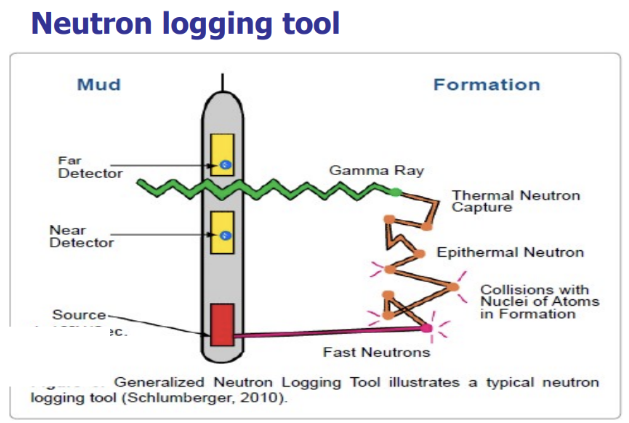
\includegraphics[width=0.8\linewidth]{img/Neutronová karotáž.png}
    \caption{Neutronová karotáž}
\end{figure}

\subsection{Metody využívající zpětný odraz gama}

\textbf{Stanovení obsahu popela v uhlí:}

Zpětný rozptyl záření gama se například využívá pro stanovení obsahu popela v uhlí, kde využívá energetické závislosti píku zpětně odraženého gama záření. Princip je vlastně identický jako u gamma-gamma karotáže:

\begin{itemize}
    \item[1)] Emitované fotony interagují s materiálem (uhlí) $\rightarrow$ Comptonův rozptyl, část fotonů odražena zpět.
    \item[2)] Detektorem měřím intenzitu odražených fotonů.
    \item[3)] Míra rozptylu závisí na hustotě elektronů v materiálu, což je ovlivněno atomovým složením a hustotou.
    \item[-] uhlí -- především H, C, O, N a S \& popel $\rightarrow$ těžší sloučeniny -- oxidy křemíku, hliníku, železa, vápníku etc.
    \item[-] popel -- větší $Z$ $\rightarrow$ více elektronů \& větší hustota $\rightarrow$ větší elektronová hustota $\rightarrow$ pravděpodobnější rozptyl a absorpce $\rightarrow$ pokles intenzity.
    \item[4)] Naopak tam, kde je hodně uhlí a málo popela $\rightarrow$ vysoká intenzita odraženého gamma.
\end{itemize}

Řízení přívodu uhlí do elektrárny:

\begin{itemize}
     \item Provoz elektrárny vyžaduje přívod uhlí o specifické výhřevnosti. V případě jakékoliv odchylky může dojít ke ztrátě výkonu nebo dokonce k výpadku kotle.
     \item Obsah popela uhelného uhlí a výhřevnost je sledována před plněním sila, aby byla zajištěna dostatečná kvalita uhlí pro správný provoz kotle.
     \item  V případě, že on-line bilance kvality uhlí neodpovídají požadavkům kotle, lze do některých sil nakládat uhlí různé kvality.
    \item  Parametry veškerého uhlí, které je pro kotel k dispozici, slouží obsluze k úpravě pracovních parametrů kotle podle potřeby.
\end{itemize}

\textbf{In-situ analýza a kontrola těžby:}

V některých případech je možné gamma záření využít pro in-situ analýzu hornin během těžby. Speciální zařízení mohou měřit intenzitu gamma záření přímo na místě a poskytovat okamžitou zpětnou vazbu o kvalitě rudy. To umožňuje optimalizovat proces těžby a zpracování nerostů tím, že těžba může být řízena na základě skutečné kvality vytěženého materiálu.

\begin{itemize}
    \item In-situ leaching: roztok kyseliny rozpouští uran z rudy $\rightarrow$ následně je monitorována koncentrace uranu v roztoku, optimalizováno pro co nejmenší dopasd na ŽP a efektivnost práce.
    \item Lze také při klasické těžbě - monitoruji jednotlivé "vozíky" s rudou.
\end{itemize}

%Nejsem si jistý, jestli se měří radiaktivní izotopy (uran, thorium ...) -- tzn. pasivní metoda, nebo se sleduje také rozptyl (nebo charakteristické záření?) asi by šlo sestrojit různé metody.

Pásová analýza (nebo-li analýza materiálu v průběhu toho co mi běží na běžícím páse a mohu tak online stanovovat kvalitu uhlí): Metoda stanovení obsahu popela v uhlí pomocí gama záření využívá principu měření intenzity gama záření, které prochází vzorkem uhlí. Popel v uhlí má specifické vlastnosti, které ovlivňují absorpci a rozptyl gama záření. Na základě těchto změn lze určit obsah popela ve vzorku.

\textbf{Analýza kalů (slurry analysis):} 

Gama záření se používá k měření koncentrace pevných částic v kalu. Princip je podobný jako u měření obsahu popela v uhlí či stanovování hustoty, ale také se využívá při loggingu (karotáž, viz Vrtání do země, psáno výše).

\underline{Pozn.:} Jak odhalím podíl prvku ve sloučenině? Pokud je prvek dostatečně těžký, resp. všechny prvky, co jsou ve sloučenině, není nic jednoduššího než použít RFA a využít detekci charakteristického RTG záření. Pokud je ovšem třeba jen jeden prvek ze dvou, tak to jde taky tak udělat a od celkového množství odečtu to, co naměřím, čímž získám zbytek. Možností je také využít rozdílu mezi fotoefektem a comptonovým roztpylem, kde fotoefekt má vyšší pravděpodobnost pro těžší atomy, a proto se na celkovém podílu reakcí více podílí pro lehké atomy Comptonovův rozptyl. Poslední možností je, pokud to umožňuje, využít neutronovou aktivační analýzu.

\newpage
\mbox{}
\newpage
